\documentclass[12pt]{article}

\usepackage[portuguese]{babel}
\usepackage[utf8]{inputenc}
\usepackage{amsmath}
\usepackage{commath}
\usepackage[alf]{abntex2cite}
\usepackage{indentfirst}
\usepackage{graphicx}
\usepackage{multicol,lipsum}
\usepackage{subfig}
\usepackage{geometry}
\usepackage[alf]{abntex2cite}


\geometry{
	paper = a4paper,
    inner = 3cm,
    outer = 3cm,
    top = 2cm,
    bottom = 2cm
}

\begin{document}
%\maketitle

\onehalfspacing

\begin{titlepage}
	\begin{center}

		\Huge{Universidade Federal de Alagoas}\\
		\large{Instituto de Computação}\\ 
		\large{Laboratório de Computação Científica e Análise Numérica}\\ 
        \vspace{220pt}
        \textbf{\LARGE{Relatório de acompanhamento de pesquisa}}\\
		%\title{{\large{Título}}}
		\vspace{3,5cm}
	\end{center}
	
	\begin{flushleft}
		\begin{tabbing}
			Aluno: Danilo Fernandes Costa\\
			Professor orientador: Alejandro Frery\\
	\end{tabbing}
 \end{flushleft}
	\vspace{1cm}
	
	\begin{center}
		\vspace{\fill}
			 Dezembro\\
		 2018
			\end{center}
\end{titlepage}

\section{Resumo}

O presente relatório visa averiguar se o comportamento observado no relatório anterior acerca das similaridades dos dados de regiões de vegetação em relação aos retroespalhadores \textit{trihedral}, \textit{dihedral} e \textit{random volume} extende-se para outras imagens. Para tal, utilizou-se dados, obtidos em UAVSAR, referentes a regiões de Ponderosa Forest, Califórnia, EUA e Slumgullion, Colorado, EUA. 

Além disso, são analisados os histogramas das similaridades de regiões de vegetação em relação aos retroespalhadores prototípicos \textit{narrow dihedral}, \textit{cylinder}, \textit{dipole}, \textit{left helix}, \textit{right helix}, \textit{+1/4-wave} e \textit{-1/4-wave}, cujas matrizes de Kennaugh são respectivamente:

\[K_{nd} =
\begin{pmatrix}
5/8 & 3/8 & 0 & 0\\
3/8 & 5/8 & 0 & 0\\
0 & 0 & -1/2 & 0\\
0 & 0 & 0 & 1/2
\end{pmatrix},
K_{c} =
\begin{pmatrix}
5/8 & 3/8 & 0 & 0\\
3/8 & 5/8 & 0 & 0\\
0 & 0 & 1/2 & 0\\
0 & 0 & 0 & -1/2\\
\end{pmatrix}
,\]

\[K_d=
\begin{pmatrix}
1 & -1 & 0 & 0\\
-1 & 1 & 0 & 0\\
0 & 0 & 0 & 0\\
0 & 0 & 0 & 0\\
\end{pmatrix},
K_{lh}=
\begin{pmatrix}
1 & 0 & 0 & -1\\
0 & 0 & 0 & 0\\
0 & 0 & 0 & 0\\
-1 & 0 & 0 & 1\\
\end{pmatrix},
K_{rh}=
\begin{pmatrix}
1 & 0 & 0 & 1\\
0 & 0 & 0 & 0\\
0 & 0 & 0 & 0\\
1 & 0 & 0 & 1\\
\end{pmatrix}
,\]

\[K_{+1/4}=
\begin{pmatrix}
1 & 0 & 0 & 0\\
0 & 1 & 0 & 0\\
0 & 0 & 0 & 1\\
0 & 0 & 1 & 0\\
\end{pmatrix},
K_{+1/4}=
\begin{pmatrix}
1 & 0 & 0 & 0\\
0 & 1 & 0 & 0\\
0 & 0 & 0 & -1\\
0 & 0 & -1 & 0\\
\end{pmatrix}
.\]

\section{Histogramas de similaridades dos dados de regiões de Ponderosa Forest e Slumgullion}

As figuras \ref{fig:pond} e \ref{fig:slum} exibem as regiões de vegetação cujos dados foram calculados as similaridades em relação aos retroespalhadores prototípicos \textit{trihedral}, \textit{dihedral} e \textit{random volume}.
\newpage

\begin{figure}[!h]
    \centering
    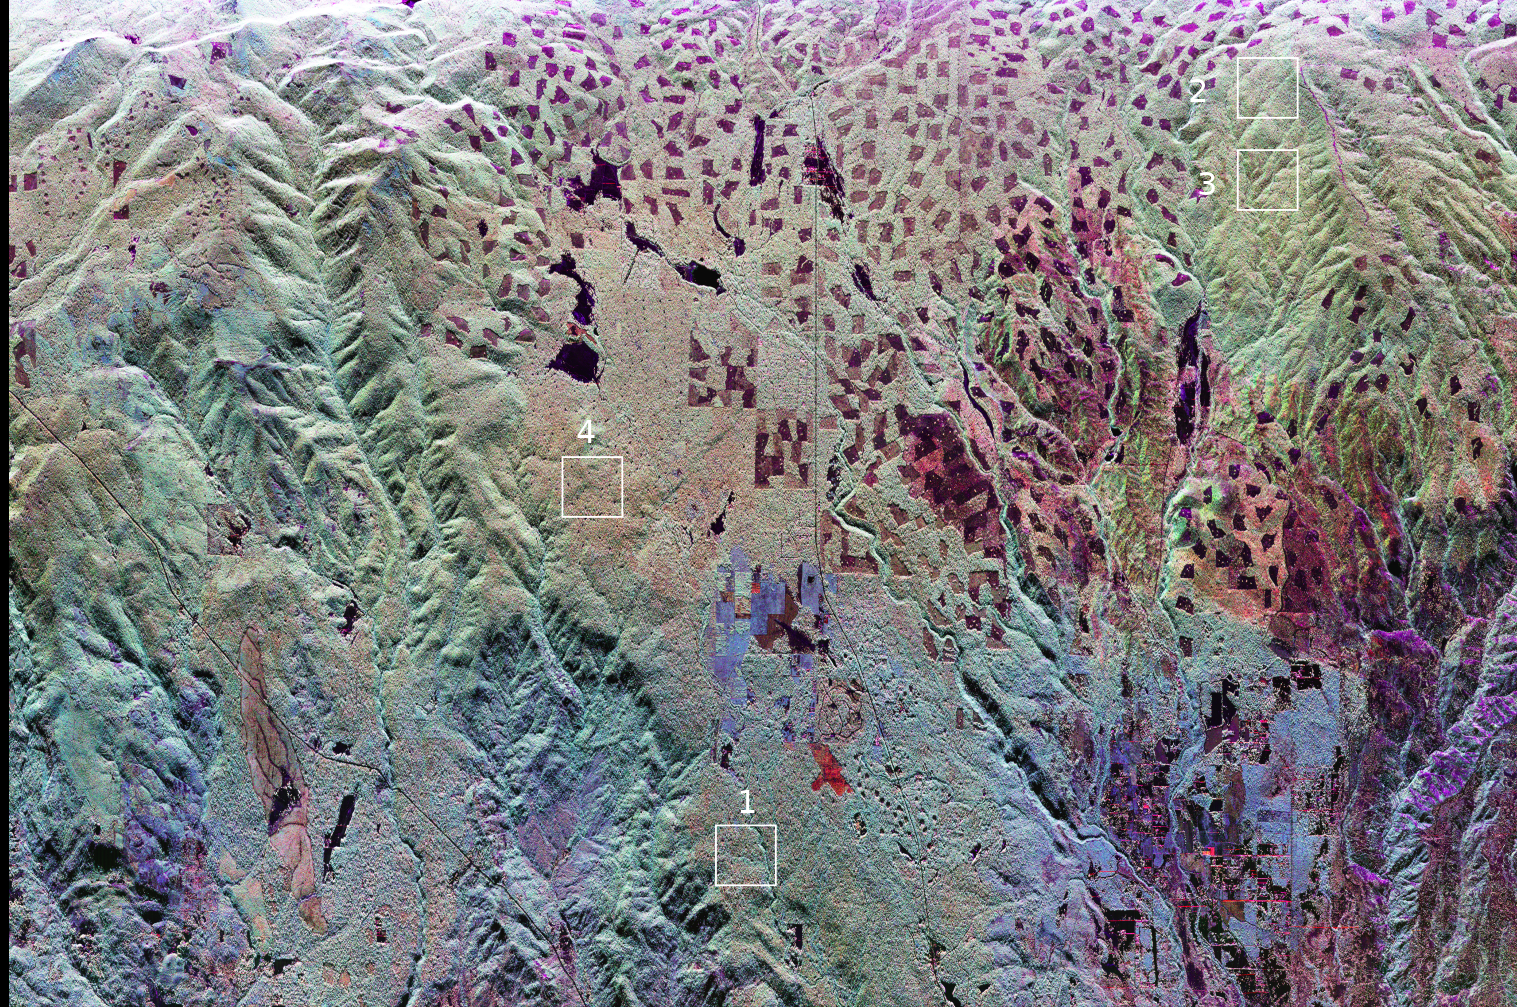
\includegraphics[width = \linewidth]{../../Images/Report_18_12_20/ponder.png}
    \caption{Ponderosa Forest, Califórnia, EUA}
    \label{fig:pond}
\end{figure}

\begin{figure}[!h]
    \centering
    \includegraphics[width = 0.9\linewidth]{../../Images/Report_18_12_20/slum.png}
    \caption{Slumgullion, Colorado, EUA}
    \label{fig:slum}
\end{figure}

As figuras \ref{fig:pond_tri_r1}, \ref{fig:pond_tri_r2}, \ref{fig:pond_tri_r3}, \ref{fig:pond_tri_r4}, \ref{fig:slum_tri_r1}, \ref{fig:slum_tri_r2} e \ref{fig:slum_tri_r3} apresentam os histogramas das similaridades das regiões selecionadas nas figuras \ref{fig:pond} e \ref{fig:slum} em relação ao retroespalhador prototípico \textit{trihedral}. É observável a relativa proximidade com os resultados obtidos no relatório anterior, contudo houve um aumento na média e na assimetria dos histogramas. Desconfia-se que a causa disto esteja relacionada com o grau de vegetação.

\begin{figure}[!h]
    \centering
    \includegraphics[width = \linewidth]{../../Images/Report_18_12_20/ponder_tri_region1.png}
    \caption{Região 1, Ponderosa Forest}
    \label{fig:pond_tri_r1}
\end{figure}

\begin{figure}[!h]
    \centering
    \includegraphics[width = \linewidth]{../../Images/Report_18_12_20/ponder_tri_region2.png}
    \caption{Região 2, Ponderosa Forest}
    \label{fig:pond_tri_r2}
\end{figure}

\begin{figure}[!h]
    \centering
    \vspace{0.1\linewidth}
    \includegraphics[width = \linewidth]{../../Images/Report_18_12_20/ponder_tri_region3.png}
    \caption{Região 3, Ponderosa Forest}
    \label{fig:pond_tri_r3}
\end{figure}

\begin{figure}[!h]
    \centering
    \vspace{0.1\linewidth}
    \includegraphics[width = \linewidth]{../../Images/Report_18_12_20/ponder_tri_region4.png}
    \caption{Região 4, Ponderosa Forest}
    \label{fig:pond_tri_r4}
\end{figure}

\begin{figure}[!h]
    \centering
    \vspace{0.1\linewidth}
    \includegraphics[width = \linewidth]{../../Images/Report_18_12_20/slum_tri_region1.png}
    \caption{Região 1, Slumgullion}
    \label{fig:slum_tri_r1}
\end{figure}

\begin{figure}[!h]
    \centering
    \vspace{0.1\linewidth}
    \includegraphics[width = \linewidth]{../../Images/Report_18_12_20/slum_tri_region2.png}
    \caption{Região 2, Slumgullion}
    \label{fig:slum_tri_r2}
\end{figure}

\begin{figure}[!h]
    \centering
    \includegraphics[width = \linewidth]{../../Images/Report_18_12_20/slum_tri_region3.png}
    \caption{Região 3, Slumgullion}
    \label{fig:slum_tri_r3}
\end{figure}


As figuras \ref{fig:pond_di_r1}, \ref{fig:pond_di_r2}, \ref{fig:pond_di_r3}, \ref{fig:pond_di_r4}, \ref{fig:slum_di_r1}, \ref{fig:slum_di_r2} e \ref{fig:slum_di_r3} apresentam os histogramas das similaridades das regiões selecionadas nas figuras \ref{fig:pond} e \ref{fig:slum} em relação ao retroespalhador prototípico \textit{dihedral}. É observável a relativa proximidade com os resultados obtidos no relatório anterior.

\begin{figure}[!h]
    \centering
    \vspace{0.05\linewidth}
    \includegraphics[width = \linewidth]{../../Images/Report_18_12_20/ponder_di_region1.png}
    \caption{Região 1, Ponderosa Forest}
    \label{fig:pond_di_r1}
\end{figure}

\begin{figure}[!h]
    \centering
    \vspace{0.08\linewidth}
    \includegraphics[width = \linewidth]{../../Images/Report_18_12_20/ponder_di_region2.png}
    \caption{Região 2, Ponderosa Forest}
    \label{fig:pond_di_r2}
\end{figure}

\begin{figure}[!h]
    \centering
    \vspace{0.1\linewidth}
    \includegraphics[width = \linewidth]{../../Images/Report_18_12_20/ponder_di_region3.png}
    \caption{Região 3, Ponderosa Forest}
    \label{fig:pond_di_r3}
\end{figure}

\begin{figure}[!h]
    \centering
    \vspace{0.1\linewidth}
    \includegraphics[width = \linewidth]{../../Images/Report_18_12_20/ponder_di_region4.png}
    \caption{Região 4, Ponderosa Forest}
    \label{fig:pond_di_r4}
\end{figure}

\begin{figure}[!h]
    \centering
    \vspace{0.1\linewidth}
    \includegraphics[width = \linewidth]{../../Images/Report_18_12_20/slum_di_region1.png}
    \caption{Região 1, Slumgullion}
    \label{fig:slum_di_r1}
\end{figure}

\begin{figure}[!h]
    \centering
    \vspace{0.1\linewidth}
    \includegraphics[width = \linewidth]{../../Images/Report_18_12_20/slum_di_region2.png}
    \caption{Região 2, Slumgullion}
    \label{fig:slum_di_r2}
\end{figure}

\begin{figure}[!h]
    \centering
    \vspace{0.1\linewidth}
    \includegraphics[width = \linewidth]{../../Images/Report_18_12_20/slum_di_region3.png}
    \caption{Região 3, Slumgullion}
    \label{fig:slum_di_r3}
\end{figure}

As figuras \ref{fig:pond_rv_r1}, \ref{fig:pond_rv_r2}, \ref{fig:pond_rv_r3}, \ref{fig:pond_rv_r4}, \ref{fig:slum_rv_r1}, \ref{fig:slum_rv_r2} e \ref{fig:slum_rv_r3} apresentam os histogramas das similaridades das regiões selecionadas nas figuras \ref{fig:pond} e \ref{fig:slum} em relação ao retroespalhador prototípico \textit{random volume}. É observável a relativa proximidade com os resultados obtidos no relatório anterior, entretanto, é nítido o aumento da média e da assimetria dos histogramas relativos aos dados de Ponderosa Forest.  

\begin{figure}[!h]
    \centering
    \includegraphics[width = 0.95\linewidth]{../../Images/Report_18_12_20/ponder_rv_region1.png}
    \caption{Região 1, Ponderosa Forest}
    \label{fig:pond_rv_r1}
\end{figure}

\begin{figure}[!h]
    \centering
    \includegraphics[width = 0.95\linewidth]{../../Images/Report_18_12_20/ponder_rv_region2.png}
    \caption{Região 2, Ponderosa Forest}
    \label{fig:pond_rv_r2}
\end{figure}

\begin{figure}[!h]
    \centering
    \vspace{0.1\linewidth}
    \includegraphics[width = \linewidth]{../../Images/Report_18_12_20/ponder_rv_region3.png}
    \caption{Região 3, Ponderosa Forest}
    \label{fig:pond_rv_r3}
\end{figure}

\begin{figure}[!h]
    \centering
    \vspace{0.1\linewidth}
    \includegraphics[width = \linewidth]{../../Images/Report_18_12_20/ponder_rv_region4.png}
    \caption{Região 4, Ponderosa Forest}
    \label{fig:pond_rv_r4}
\end{figure}

\begin{figure}[!h]
    \centering
    \vspace{0.1\linewidth}
    \includegraphics[width = \linewidth]{../../Images/Report_18_12_20/slum_rv_region1.png}
    \caption{Região 1, Slumgullion}
    \label{fig:slum_rv_r1}
\end{figure}

\begin{figure}[!h]
    \centering
    \vspace{0.1\linewidth}
    \includegraphics[width = \linewidth]{../../Images/Report_18_12_20/slum_rv_region2.png}
    \caption{Região 2, Slumgullion}
    \label{fig:slum_rv_r2}
\end{figure}

\begin{figure}[!h]
    \centering
    \includegraphics[width = \linewidth]{../../Images/Report_18_12_20/slum_rv_region3.png}
    \caption{Região 2, Slumgullion}
    \label{fig:slum_rv_r3}
\end{figure}

\section{Histogramas de similaridades em relação a outros retroespalhadores prototípicos}

Para a construção dos histogramas foram utilizadas as similaridades em relação aos retroespalhadores prototípicos \textit{narrow dihedral}, \textit{cylinder}, \textit{dipole}, \textit{left helix}, \textit{right helix}, \textit{+1/4-wave} e \textit{-1/4-wave} obtidas para os dados das regiões de vegetação de Guatemala utilizadas no relatório anterior e expostas na figura \ref{fig:guatemala}

\begin{figure}[!h]
    \centering
    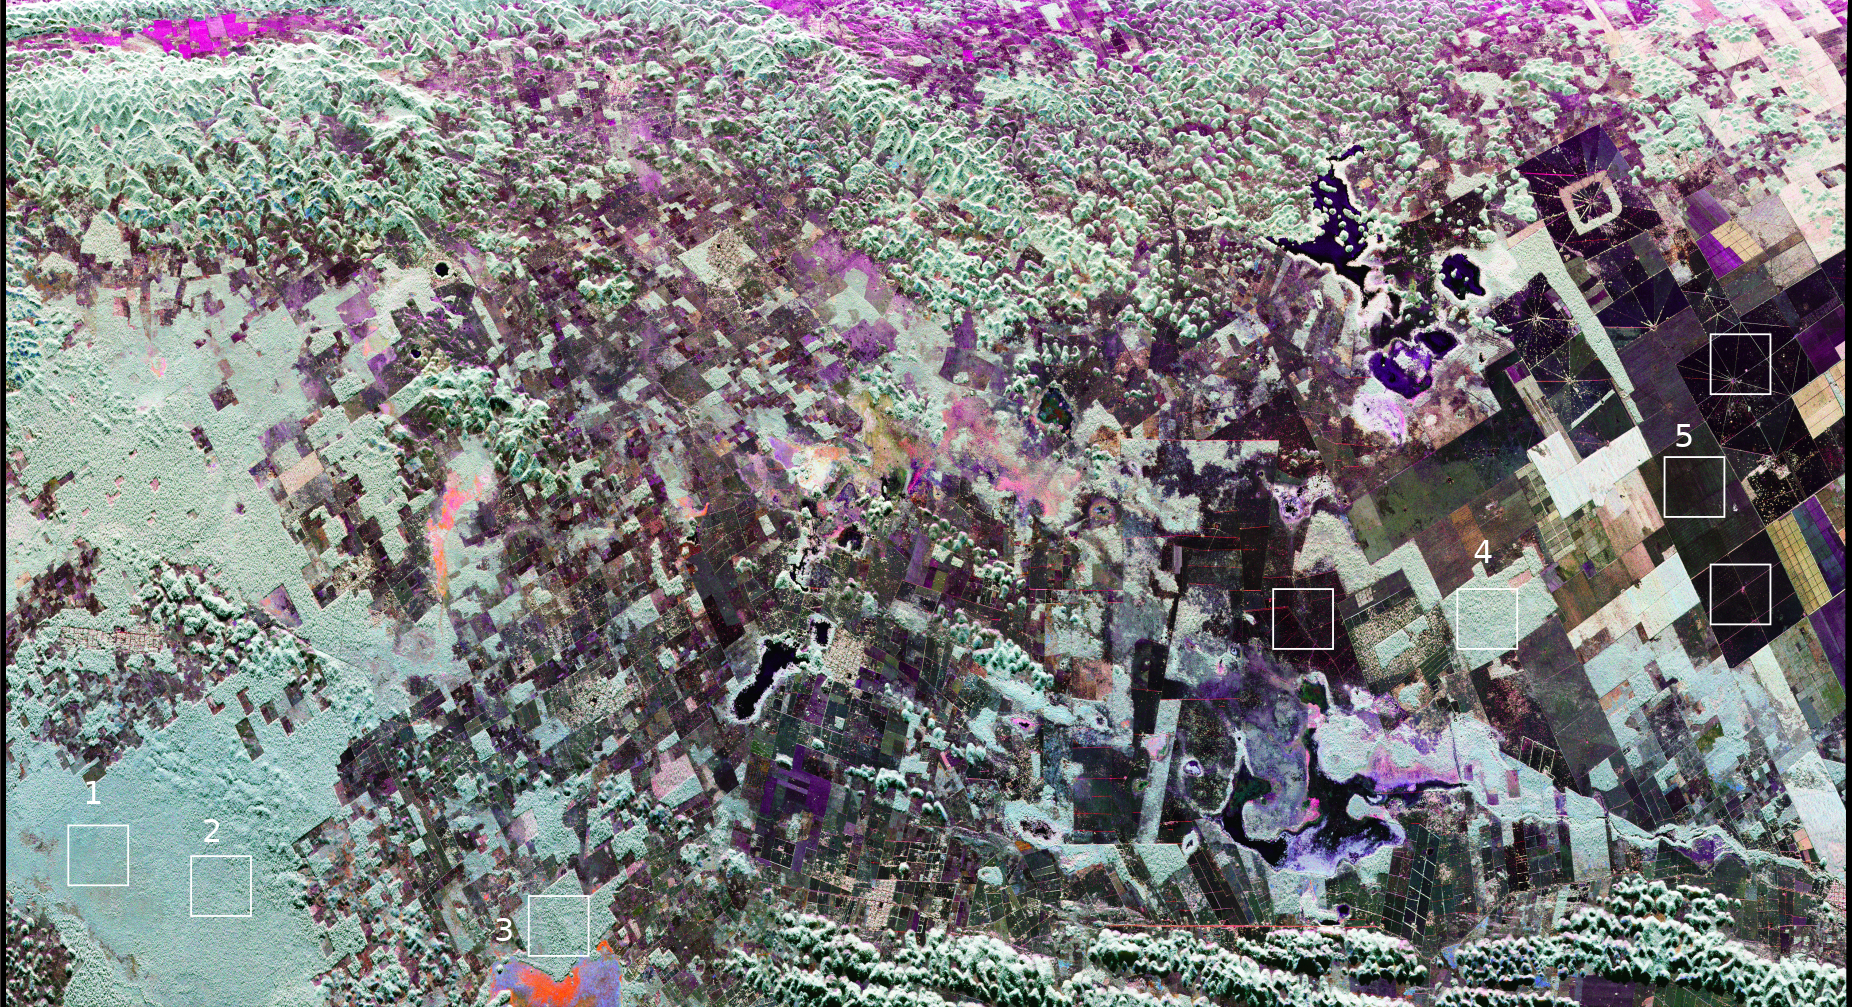
\includegraphics[width = \linewidth]{../../Images/Report_18_12_20/guatemala2.png}
    \caption{Regiões de vegetação em Guatemala selecionadas para análise}
    \label{fig:guatemala}
\end{figure}

As figuras \ref{fig:nd_r1}, \ref{fig:nd_r2}, \ref{fig:nd_r3}, \ref{fig:nd_r4} e \ref{fig:nd_r5} apresentam os histogramas das similaridades dos dados dessas regiões em relação ao retroespalhador prototípico \textit{narrow dihedral}. É observável o ajuste à distribuição Gama e a relativa proximidade entre os parâmetros estimados, com exceção da região 5.

\begin{figure}[!h]
    \centering
    \includegraphics[width = \linewidth]{../../Images/Report_18_12_20/nd_region1.png}
    \caption{Região 1}
    \label{fig:nd_r1}
\end{figure}

\begin{figure}[!h]
    \centering
    \includegraphics[width = \linewidth]{../../Images/Report_18_12_20/nd_region2.png}
    \caption{Região 2}
    \label{fig:nd_r2}
\end{figure}

\begin{figure}[!h]
    \centering
    \vspace{0.1\linewidth}
    \includegraphics[width = \linewidth]{../../Images/Report_18_12_20/nd_region3.png}
    \caption{Região 3}
    \label{fig:nd_r3}
\end{figure}

\begin{figure}[!h]
    \centering
    \vspace{0.1\linewidth}
    \includegraphics[width = \linewidth]{../../Images/Report_18_12_20/nd_region4.png}
    \caption{Região 4}
    \label{fig:nd_r4}
\end{figure}

\begin{figure}[!h]
    \centering
    \includegraphics[width = \linewidth]{../../Images/Report_18_12_20/nd_region5.png}
    \caption{Região 5}
    \label{fig:nd_r5}
\end{figure}

As figuras \ref{fig:cy_r1}, \ref{fig:cy_r2}, \ref{fig:cy_r3}, \ref{fig:cy_r4} e \ref{fig:cy_r5} apresentam os histogramas das similaridades dos dados das regiões 1 à 5 em relação ao retroespalhador prototípico \textit{cylinder}. É observável o ajuste à distribuição Normal e a relativa proximidade entre os parâmetros estimados.

\begin{figure}[!h]
    \centering
    \vspace{0.05\linewidth}
    \includegraphics[width = \linewidth]{../../Images/Report_18_12_20/cy_region1.png}
    \caption{Região 1}
    \label{fig:cy_r1}
\end{figure}

\begin{figure}[!h]
    \centering
    \vspace{0.08\linewidth}
    \includegraphics[width = \linewidth]{../../Images/Report_18_12_20/cy_region2.png}
    \caption{Região 2}
    \label{fig:cy_r2}
\end{figure}

\begin{figure}[!h]
    \centering
    \vspace{0.1\linewidth}
    \includegraphics[width = \linewidth]{../../Images/Report_18_12_20/cy_region3.png}
    \caption{Região 3}
    \label{fig:cy_r3}
\end{figure}

\begin{figure}[!h]
    \centering
    \vspace{0.1\linewidth}
    \includegraphics[width = \linewidth]{../../Images/Report_18_12_20/cy_region4.png}
    \caption{Região 4}
    \label{fig:cy_r4}
\end{figure}

\begin{figure}[!h]
    \centering
    \vspace{0.1\linewidth}
    \includegraphics[width = \linewidth]{../../Images/Report_18_12_20/cy_region5.png}
    \caption{Região 5}
    \label{fig:cy_r5}
\end{figure}

As figuras \ref{fig:dip_r1}, \ref{fig:dip_r2}, \ref{fig:dip_r3}, \ref{fig:dip_r4} e \ref{fig:dip_r5} apresentam os histogramas das similaridades dos dados das regiões 1 à 5 em relação ao retroespalhador prototípico \textit{dipole}. É observável o ajuste à distribuição Gama e a relativa proximidade entre os parâmetros estimados, com exceção do histograma da figura \ref{fig:dip_r5}.

\begin{figure}[!h]
    \centering
    \includegraphics[width = \linewidth]{../../Images/Report_18_12_20/dip_region1.png}
    \caption{Região 1}
    \label{fig:dip_r1}
\end{figure}

\begin{figure}[!h]
    \centering
    \includegraphics[width = \linewidth]{../../Images/Report_18_12_20/dip_region2.png}
    \caption{Região 2}
    \label{fig:dip_r2}
\end{figure}

\begin{figure}[!h]
    \centering
    \vspace{0.1\linewidth}
    \includegraphics[width = \linewidth]{../../Images/Report_18_12_20/dip_region3.png}
    \caption{Região 3}
    \label{fig:dip_r3}
\end{figure}

\begin{figure}[!h]
    \centering
    \vspace{0.1\linewidth}
    \includegraphics[width = \linewidth]{../../Images/Report_18_12_20/dip_region4.png}
    \caption{Região 4}
    \label{fig:dip_r4}
\end{figure}

\begin{figure}[!h]
    \centering
    \includegraphics[width = \linewidth]{../../Images/Report_18_12_20/dip_region5.png}
    \caption{Região 5}
    \label{fig:dip_r5}
\end{figure}

As figuras \ref{fig:lh_r1}, \ref{fig:lh_r2}, \ref{fig:lh_r3}, \ref{fig:lh_r4} e \ref{fig:lh_r5} apresentam os histogramas das similaridades dos dados das regiões 1 à 5 em relação ao retroespalhador prototípico \textit{left helix}. É observável o ajuste a distribuição Gama e a relativa proximidade entre os parâmetros estimados, com execeção do histograma da figura \ref{fig:lh_r5}.

\begin{figure}[!h]
    \centering
    \includegraphics[width = \linewidth]{../../Images/Report_18_12_20/lh_region1.png}
    \caption{Região 1}
    \label{fig:lh_r1}
\end{figure}

\begin{figure}[!h]
    \centering
    \vspace{0.1\linewidth}
    \includegraphics[width = \linewidth]{../../Images/Report_18_12_20/lh_region2.png}
    \caption{Região 2}
    \label{fig:lh_r2}
\end{figure}

\begin{figure}[!h]
    \centering
    \vspace{0.1\linewidth}
    \includegraphics[width = \linewidth]{../../Images/Report_18_12_20/lh_region3.png}
    \caption{Região 3}
    \label{fig:lh_r3}
\end{figure}

\begin{figure}[!h]
    \centering
    \vspace{0.10\linewidth}
    \includegraphics[width = \linewidth]{../../Images/Report_18_12_20/lh_region4.png}
    \caption{Região 4}
    \label{fig:lh_r4}
\end{figure}

\begin{figure}[!h]
    \centering
    \vspace{0.1\linewidth}
    \includegraphics[width = \linewidth]{../../Images/Report_18_12_20/lh_region5.png}
    \caption{Região 5}
    \label{fig:lh_r5}
\end{figure}

As figuras \ref{fig:rh_r1}, \ref{fig:rh_r2}, \ref{fig:rh_r3}, \ref{fig:rh_r4} e \ref{fig:rh_r5} apresentam os histogramas das similaridades dos dados das regiões 1 à 5 em relação ao retroespalhador prototípico \textit{right helix}. É observável o ajuste a distribuição Gama e a relativa proximidade entre os parâmetros estimados, com execeção do histograma da figura \ref{fig:rh_r5}.

\begin{figure}[!h]
    \centering
    \includegraphics[width = \linewidth]{../../Images/Report_18_12_20/rh_region1.png}
    \caption{Região 1}
    \label{fig:rh_r1}
\end{figure}

\begin{figure}[!h]
    \centering
    \includegraphics[width = \linewidth]{../../Images/Report_18_12_20/rh_region2.png}
    \caption{Região 2}
    \label{fig:rh_r2}
\end{figure}

\begin{figure}[!h]
    \centering
    \vspace{0.1\linewidth}
    \includegraphics[width = \linewidth]{../../Images/Report_18_12_20/rh_region3.png}
    \caption{Região 3}
    \label{fig:rh_r3}
\end{figure}

\begin{figure}[!h]
    \centering
    \vspace{0.1\linewidth}
    \includegraphics[width = \linewidth]{../../Images/Report_18_12_20/rh_region4.png}
    \caption{Região 4}
    \label{fig:rh_r4}
\end{figure}

\begin{figure}[!h]
    \centering
    \includegraphics[width = \linewidth]{../../Images/Report_18_12_20/rh_region5.png}
    \caption{Região 5}
    \label{fig:rh_r5}
\end{figure}

As figuras \ref{fig:pwv_r1}, \ref{fig:pwv_r2}, \ref{fig:pwv_r3}, \ref{fig:pwv_r4} e \ref{fig:pwv_r5} apresentam os histogramas das similaridades dos dados das regiões selecionadas  em relação ao retroespalhador prototípico \textit{+1/4-wave}. É observável o ajuste a distribuição Gama e a relativa proximidade entre os parâmetros estimados, com execeção do histograma da figura \ref{fig:pwv_r5}.

\begin{figure}[!h]
    \centering
    \includegraphics[width = \linewidth]{../../Images/Report_18_12_20/pwv_region1.png}
    \caption{Região 1}
    \label{fig:pwv_r1}
\end{figure}

\begin{figure}[!h]
    \centering
    \vspace{0.1\linewidth}
    \includegraphics[width = \linewidth]{../../Images/Report_18_12_20/pwv_region2.png}
    \caption{Região 2}
    \label{fig:pwv_r2}
\end{figure}

\begin{figure}[!h]
    \centering
    \vspace{0.1\linewidth}
    \includegraphics[width = \linewidth]{../../Images/Report_18_12_20/pwv_region3.png}
    \caption{Região 3}
    \label{fig:pwv_r3}
\end{figure}

\begin{figure}[!h]
    \centering
    \vspace{0.1\linewidth}
    \includegraphics[width = \linewidth]{../../Images/Report_18_12_20/pwv_region4.png}
    \caption{Região 4}
    \label{fig:pwv_r4}
\end{figure}

\begin{figure}[!h]
    \centering
    \vspace{0.1\linewidth}
    \includegraphics[width = \linewidth]{../../Images/Report_18_12_20/pwv_region5.png}
    \caption{Região 5}
    \label{fig:pwv_r5}
\end{figure}

As figuras \ref{fig:nwv_r1}, \ref{fig:nwv_r2}, \ref{fig:nwv_r3}, \ref{fig:nwv_r4} e \ref{fig:nwv_r5} apresentam os histogramas das similaridades dos dados das regiões selecionadas  em relação ao retroespalhador prototípico \textit{-1/4-wave}. É observável o ajuste a distribuição Gama e a relativa proximidade entre os parâmetros estimados, com execeção do histograma da figura \ref{fig:nwv_r5}.

\begin{figure}[!h]
    \centering
    \includegraphics[width = \linewidth]{../../Images/Report_18_12_20/nwv_region1.png}
    \caption{Região 1}
    \label{fig:nwv_r1}
\end{figure}

\begin{figure}[!h]
    \centering
    \includegraphics[width = \linewidth]{../../Images/Report_18_12_20/nwv_region2.png}
    \caption{Região 2}
    \label{fig:nwv_r2}
\end{figure}

\begin{figure}[!h]
    \centering
    \vspace{0.1\linewidth}
    \includegraphics[width = \linewidth]{../../Images/Report_18_12_20/nwv_region3.png}
    \caption{Região 3}
    \label{fig:nwv_r3}
\end{figure}

\begin{figure}[!h]
    \centering
    \vspace{0.1\linewidth}
    \includegraphics[width = \linewidth]{../../Images/Report_18_12_20/nwv_region4.png}
    \caption{Região 4}
    \label{fig:nwv_r4}
\end{figure}

\begin{figure}[!h]
    \centering
    \vspace{0.1\linewidth}
    \includegraphics[width = \linewidth]{../../Images/Report_18_12_20/nwv_region5.png}
    \caption{Região 5}
    \label{fig:nwv_r5}
\end{figure}


\end{document}
